% ========================================
% Paper #67 of the 0-Sphere Model series (DRAFT)
% The Spheroidal Hose: A Kinematic Picture of the 0-Sphere Electron Consistent with Special and General Relativity
% Author: Satoshi Hanamura (ORCID 0009-0000-2687-0918)
% Date  : draft of November 27, 2026
% DOI   : [pending]
% Verification script: verify67.py
% ========================================
% ========================================
% Document Class and Package Setup
% ========================================
\documentclass[%
 reprint, amsmath,amssymb, aps, prb, ]{revtex4-2}
% Basic packages
\usepackage{graphicx}
\usepackage{bm}
% Quantum-mechanics notation
\usepackage{physics}
% Hyperlinks
\usepackage[colorlinks=true,
            linkcolor=blue, filecolor=blue, urlcolor=blue, citecolor=blue]{hyperref}
% Caption settings
\usepackage{caption}
\captionsetup[figure]{
    justification=raggedright, labelfont={bf}, name={Fig.}, labelsep=period }
\captionsetup[table]{
    labelfont={bf}, name={Table}, labelsep=period }
% Equation numbering by section
\numberwithin{equation}{section}
% Typography adjustments
\tolerance=1000
\emergencystretch=1em
\hyphenpenalty=3000
\exhyphenpenalty=3000
\flushbottom
% Microtypography
\usepackage[final]{microtype}
\usepackage{ragged2e}  % for \justifying command
% Table rules (\midrule, \addlinespace, \bottomrule)
\usepackage{booktabs}
\usepackage{enumitem}
% Theorem environment
\usepackage{amsthm}
\newtheorem{theorem}{Theorem}[section]
% --- paragraph heading: run-in italic with extra top skip for block readability ---
\makeatletter
\renewcommand\paragraph{%
  \@startsection{paragraph}{4}{\z@}%
    {3mm \@plus 1ex \@minus .2ex}%   space before (block separator)
    {-1em}%                          space after (negative value keeps the heading run-in)
    {\normalfont\normalsize\itshape}}
\makeatother
% Code listings with syntax highlighting
\usepackage{listings}
\usepackage{xcolor}
% Colour definitions (light blue palette for listings)
\definecolor{backcolour}{rgb}{0.96,0.97,0.98}
\definecolor{deepblue}{rgb}{0,0,0.5}
\definecolor{deepgreen}{rgb}{0,0.5,0.3}
\definecolor{deepgray}{rgb}{0.4,0.4,0.4}
\definecolor{stringcolor}{rgb}{0.2,0.4,0.6}
% Python listing style
\lstdefinestyle{pythonstyle}{
    backgroundcolor=\color{backcolour}, commentstyle=\color{deepgreen}\itshape, keywordstyle=\color{deepblue}\bfseries, numberstyle=\tiny\color{deepgray}, stringstyle=\color{stringcolor}, basicstyle=\ttfamily\footnotesize, breakatwhitespace=false, breaklines=true, captionpos=b, keepspaces=true, numbers=left, numbersep=5pt, showspaces=false, showstringspaces=false, showtabs=false, tabsize=2, language=Python, frame=single, rulecolor=\color{deepgray} }
\lstset{style=pythonstyle}
% Internal phase notation
\newcommand{\iphase}{\theta}  % internal geometric phase = ωt/2
\usepackage{tikz}
\usetikzlibrary{arrows.meta, calc, 3d, shadings, positioning, decorations.pathmorphing}
% --- Custom Macros ---
\newcommand{\omZB}{\omega_{\text{ZB}}}
\newcommand{\EphS}{E_{\text{ph}}}
\newcommand{\Egrad}{\Delta E_{\text{AB}}}
% Fundamental 1-form
% Field strength 2-form
\newcommand{\FF}{\mathbf{F}}
% Open Wilson line
\newcommand{\WL}{\mathcal{W}}
% Hodge dual
\newcommand{\hodge}{\star}
% --- Paper-specific macros ---
\newcommand{\lamC}{\lambda_C}
\newcommand{\lbar}{\bar{\lambda}_C}

% ========================================
% Document Begin
% ========================================
\begin{document}

% ========================================
% Title, Author, and Date
% ========================================
\title{The Spheroidal Hose:\\A Kinematic Picture of the 0-Sphere Electron Consistent with Special and General Relativity}

\author{Satoshi Hanamura}
\homepage{https://orcid.org/0009-0000-2687-0918}

\date{Draft of November 27, 2026}

% ========================================
% Abstract
% ========================================
\begin{abstract}
In the 0-Sphere model the electron consists of two kernels, $A$ and $B$, between which the rest energy $E_0 = m_ec^2$ is carried back and forth.
This paper fixes the shape of the region in which that energy travels, using a single premise: the energy $E_0$, converted entirely into one photon, has the Compton wavelength $\lamC = h/m_ec$.
Holding that wavelength once on a round trip between the kernels gives their separation $d = \lamC/2$; holding it once around a circle gives the transverse radius $\lbar = \lamC/2\pi$.
The two lengths satisfy $d = \pi\lbar$, and the region is a prolate spheroid with semi-axes $\lamC/4$ and $\lbar$, which we call the hose.
A representative element of the carried energy that moves on the hose at speed $c$, with its polar angle advancing uniformly, projects onto the axis as the simple harmonic motion of the radiation gradient found in Paper \#1.
The energy identity splits into an occupation layer, whose centroid is that harmonic motion, and a quartic layer, whose cross term $\tfrac12\sin^2\theta$ is the energy in flight.
At the equator the circulating half of the energy gives the angular momentum $\hbar/2$, the magnetic moment $\mu_B$ and $g = 2$, the last without approximation.
The transverse motion is a light clock carried by the axial motion; an electron at rest has the prolate hose and an electron accelerated along the axis sees it contract by the Lorentz factor; the equatorial clock at the Compton frequency reproduces the de~Broglie wavelength $h/p$; and in a static gravitational potential all lengths stay fixed locally while the observed frequencies shift by the clock factor, giving the fractional difference $5.29\times10^{-10}$ between the Earth's surface and the GPS orbit.
The paper is kinematic: how the axial speed is fixed by the anomalous magnetic moment is outside its scope.
\end{abstract}

\maketitle

% ========================================
% Section 1: Introduction
% ========================================
\section{Introduction}

The 0-Sphere model describes the electron by three elements: a kernel $A$, a kernel $B$, and an amount of energy that is carried between them~\cite{H01,H66}. Paper \#1~\cite{H01} showed that the radiation gradient between two perfect black bodies drives this transport as a simple harmonic motion between fixed points. Paper \#66~\cite{H66} placed the kernels at a separation $\lamC/2$ and assigned to the transport a subluminal speed, so that the internal oscillation of the electron is a Zitterbewegung at an X-ray frequency rather than at the frequency $2m_ec^2/h$ of the Dirac theory.

Two questions of geometry were left open by these papers. The first is why the separation of the kernels should be $\lamC/2$. The second is where the energy travels while it is between the kernels, and at what speed. The second question matters for relativity: an element of energy that is light should move at $c$, while the transport it accomplishes along the axis is slower. A helical trajectory between the kernels was introduced in Paper \#51~\cite{H51} to describe this transport; the present paper fixes the surface on which such a helix lies.

The answer proposed here is a prolate spheroid, which we call the hose (Fig.~\ref{fig:hose}). Its two semi-axes follow from one premise about the Compton wavelength (Sec.~\ref{sec:premise}). An element of energy moving on it at speed $c$ projects onto the axis as the harmonic motion of Paper \#1 (Sec.~\ref{sec:hose}). The energy identity of the series separates into two layers on the hose (Sec.~\ref{sec:identity}), and the equator of the hose carries the spin quantities (Sec.~\ref{sec:ring}). The remaining sections show that the same geometry is compatible with special relativity (Secs.~\ref{sec:clock} and~\ref{sec:sr}) and with the clock effect of general relativity (Sec.~\ref{sec:gr}).

The paper is kinematic and deliberately narrow. It does not decide the value of the axial speed, which the series fixes from the anomalous magnetic moment~\cite{H10,H66}, and it treats the spin quantities at the equator only. These limits are stated in Sec.~\ref{sec:scope}. Every number in the text is reproduced by the script \texttt{verify67.py} (Appendix~\ref{app:numbers}).

The 0-Sphere model traces the electron from field theory to particle mechanics, in the spirit of smoothed-particle hydrodynamics~\cite{Monaghan1992}: the carried energy is represented by elements that move along definite paths. The word \emph{grain} below refers to one such representative element.

% ========================================
% Section 2: Premise
% ========================================
\section{One Photon, Two Lengths}
\label{sec:premise}

\paragraph{Premise.} If the rest energy $E_0 = m_ec^2$ is converted entirely into a single photon, the wavelength of that photon is the Compton wavelength~\cite{Compton1923},
\begin{equation}
E_0 = \frac{hc}{\lamC}, \qquad \lamC = \frac{h}{m_ec} = 2.4263\times10^{-12}\ \text{m}.
\label{eq:lamC}
\end{equation}
We require that the energy carried between the kernels hold this wavelength exactly once, in the lowest mode, in each of the two ways it can be held.

\paragraph{Along the axis.} A wave confined between two fixed ends has, in its lowest mode, a wavelength twice the distance between the ends, as for a pipe closed at both ends or a string fixed at both ends. Equivalently, one wavelength fits a round trip. With the kernels at $x = \mp d/2$,
\begin{equation}
2d = \lamC, \qquad d = \frac{\lamC}{2} = 1.2132\times10^{-12}\ \text{m}.
\label{eq:d}
\end{equation}
This is the separation used in Paper \#66~\cite{H66}.

\paragraph{Around the axis.} A wave that closes on a circle holds, in its lowest mode, one wavelength around the circumference, as in Bohr's condition with quantum number one~\cite{Bohr1913}. With radius $R$,
\begin{equation}
2\pi R = \lamC, \qquad R = \frac{\lamC}{2\pi} = \lbar = 3.8616\times10^{-13}\ \text{m}.
\label{eq:R}
\end{equation}

\paragraph{Consequence.} Both lengths are fixed by the same photon, so their ratio is fixed:
\begin{equation}
d = \pi \lbar, \qquad \frac{d/2}{\lbar} = \frac{\pi}{2}.
\label{eq:dpiR}
\end{equation}
The straight distance between the kernels equals half the circumference of the circle of radius $\lbar$. The hose defined in the next section is the prolate spheroid with semi-axes $d/2 = \lamC/4$ along the axis and $\lbar$ across it, and its aspect ratio is $\pi/2$.

% ========================================
% Section 3: The hose
% ========================================
\section{The Hose and Its Projection}
\label{sec:hose}

\paragraph{Surface.} Let $x$ be the axis through the kernels and $r$ the distance from it. The hose is
\begin{equation}
\frac{x^2}{(d/2)^2} + \frac{r^2}{\lbar^2} = 1.
\label{eq:spheroid}
\end{equation}
A point on it is labelled by a polar angle $\theta$, measured from kernel $A$, and an azimuth $\phi$:
\begin{equation}
x = -\frac{d}{2}\cos\theta,\quad
r = \lbar\sin\theta .
\label{eq:param}
\end{equation}
Kernel $A$ sits at $\theta = 0$, kernel $B$ at $\theta = \pi$, and the equator at $\theta = \pi/2$.

\paragraph{Motion of a grain.} A grain leaves $A$, travels on the hose, and arrives at $B$. We impose two conditions. First, the grain moves at the speed of light. Second, its polar angle advances uniformly, $\theta = \Omega t$. The first condition fixes the azimuthal rate once the second is given:
\begin{equation}
r^2\dot\phi^2 = c^2 - \Big(\frac{d}{2}\Omega\sin\theta\Big)^2 - \big(\lbar\,\Omega\cos\theta\big)^2 .
\label{eq:phidot}
\end{equation}
The grain therefore winds around the axis while it advances along it; its path is the helix drawn in Fig.~\ref{fig:hose}(a).

\paragraph{Projection.} The axial velocity of the grain is
\begin{equation}
v_x = \frac{d}{2}\,\Omega\,\sin\theta = v_p \sin\theta, \qquad v_p \equiv \frac{d}{2}\,\Omega .
\label{eq:vx}
\end{equation}
This is simple harmonic motion between the fixed points $x = \mp d/2$, which is the motion that Paper \#1 obtained from the radiation gradient between the two black bodies~\cite{H01}. Figure~\ref{fig:hose}(b) compares the projected velocity of a grain integrated from Eq.~\eqref{eq:phidot} with $\sin\theta$; they agree to $3.5\times10^{-11}$ of $v_p$. We call the axis the red line and the path on the hose the blue line. The grain on the blue line moves at $c$; its shadow on the red line moves at most at $v_p$. The present paper does not fix $v_p$; it requires only $v_p < c$, which makes the right-hand side of Eq.~\eqref{eq:phidot} positive for every $\theta$, since $\lbar\Omega = (2/\pi)v_p$.

\paragraph{Three speeds.} Three speeds appear in this paper and must be kept apart. The grain on the blue line moves at $c$, for every observer. The red line moves at most at $v_p < c$; this is an internal speed, defined in the frame in which the kernels are at rest, and over a round trip the red line returns to its starting point, so that the electron as a whole does not move. The speed $V$ of Sec.~\ref{sec:sr} is the speed of the electron as a whole, kernels included, relative to a laboratory; it is set from outside, by whatever accelerated the electron, and is zero for an electron at rest. The internal oscillation belongs to a different scope from $V$: whether the electron is accelerated or not, the red line oscillates in the electron's own frame exactly as described here, and a laboratory in which the electron moves sees only the hose contracted and the oscillation slowed by the Lorentz factor. Nothing in the construction moves faster than $c$.

\begin{figure*}[t!]
\centering
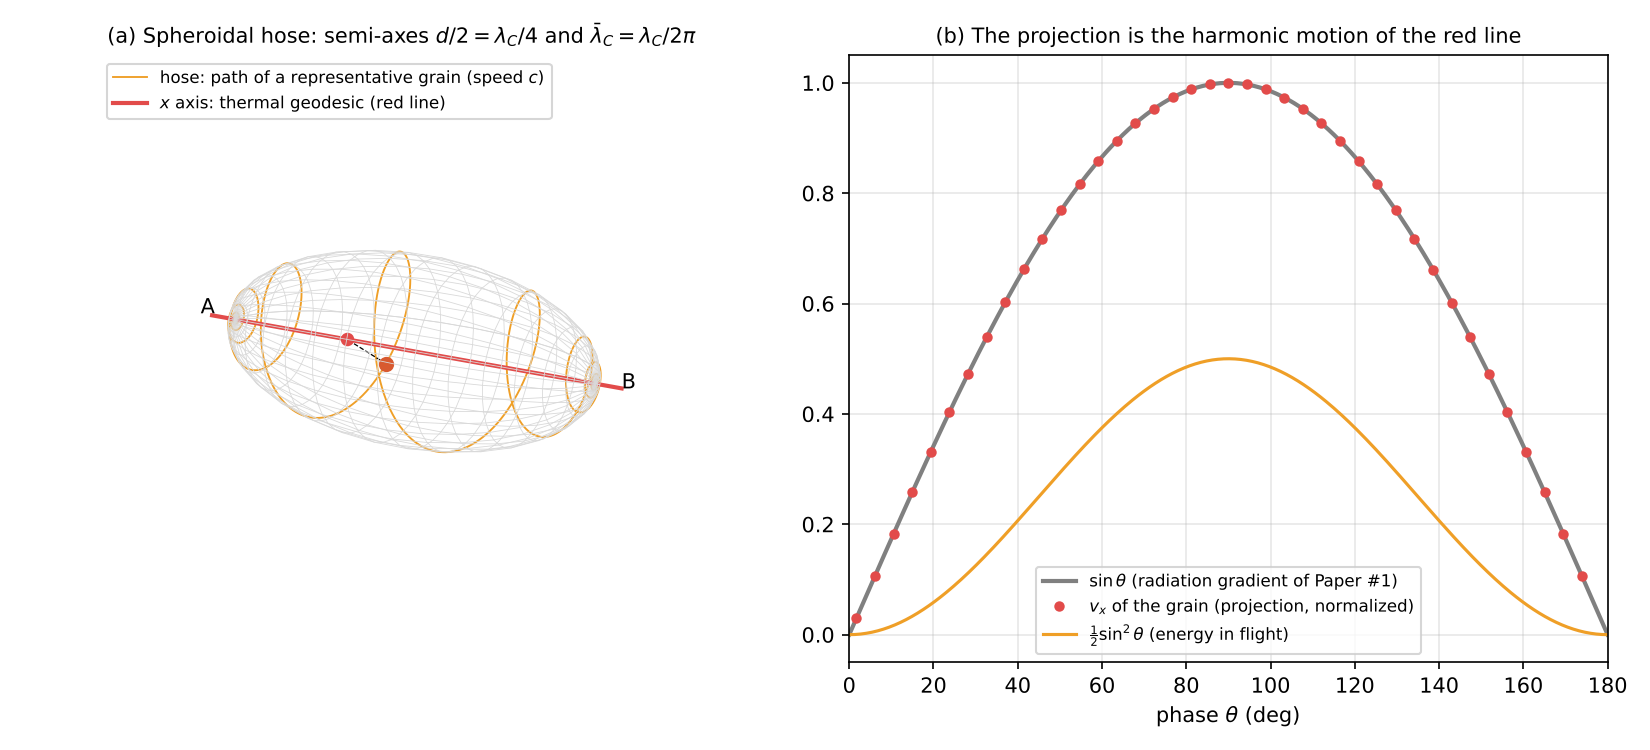
\includegraphics[width=\textwidth]{fig_hose.png}
\caption{\textbf{The spheroidal hose and the projection of a grain onto the axis}}
\label{fig:hose}
\vspace{0.4em}
\begin{minipage}{0.95\textwidth}
\justifying\small
(a) The hose is the prolate spheroid with semi-axes $d/2 = \lamC/4$ along the axis through the kernels $A$ and $B$ and $\lbar = \lamC/2\pi$ across it; its aspect ratio is $\pi/2$ [Eq.~\eqref{eq:dpiR}]. The orange curve is the path of a representative grain of the carried energy, moving at $c$ with its polar angle advancing uniformly (drawn with a small number of turns for legibility). The red line is the axis, the thermal geodesic between the kernels; the two dots joined by a dashed segment are the grain and its projection. (b) The axial velocity of the grain, obtained from the path, normalized by its maximum (dots), coincides with $\sin\theta$ (grey), the harmonic motion of Paper \#1. The orange curve is the energy in flight, $\tfrac12\sin^2\theta$ in units of $E_0$ [Eq.~\eqref{eq:quartic}], which oscillates at twice the frequency of the red line.
\end{minipage}
\end{figure*}

% ========================================
% Section 4: Identity
% ========================================
\section{Two Layers of the Energy Identity}
\label{sec:identity}

\paragraph{Occupation layer.} Write the half angle $\theta/2$ and define the two amplitudes
\begin{equation}
\psi_A = \cos\frac{\theta}{2}, \qquad \psi_B = \sin\frac{\theta}{2}, \qquad \psi_A^2 + \psi_B^2 = 1 .
\label{eq:amp}
\end{equation}
The squares $\psi_A^2$ and $\psi_B^2$ are the shares of the energy assigned to $A$ and to $B$. Placing these shares at $x = -d/2$ and $x = +d/2$, their centroid is
\begin{equation}
\bar{x} = \frac{d}{2}\big(\psi_B^2 - \psi_A^2\big) = -\frac{d}{2}\cos\theta ,
\label{eq:centroid}
\end{equation}
which is the red line of Eq.~\eqref{eq:param}. The identity $\cos^2 + \sin^2 = 1$ thus describes a single point moving from $A$ to $B$.

\paragraph{Quartic layer.} Squaring the same identity separates the energy into three parts,
\begin{equation}
1 = \underbrace{\psi_A^4}_{\text{at }A} + \underbrace{\psi_B^4}_{\text{at }B} + \underbrace{2\psi_A^2\psi_B^2}_{\text{in flight}},
\qquad 2\psi_A^2\psi_B^2 = \tfrac12\sin^2\theta .
\label{eq:quartic}
\end{equation}
This is the quartic energy of the series, whose geometric origin was given in Paper \#65~\cite{H65}. The residual energies at the kernels are $E_0\cos^4(\theta/2)$ and $E_0\sin^4(\theta/2)$, and the energy in flight is $\tfrac12E_0\sin^2\theta$.

\paragraph{The two layers are joined by the velocity.} The axial velocity of Eq.~\eqref{eq:vx} is a product of the two amplitudes,
\begin{equation}
\frac{v_x}{v_p} = \sin\theta = 2\psi_A\psi_B ,
\label{eq:vprod}
\end{equation}
so that the energy in flight is half the square of the normalized axial velocity,
\begin{equation}
\frac{E_{\text{flight}}}{E_0} = \frac12\Big(\frac{v_x}{v_p}\Big)^2 .
\label{eq:flightv}
\end{equation}
The occupation layer oscillates at the frequency of the red line, $\Omega/2\pi$ per round trip; the energy in flight, being quadratic in $v_x$, oscillates at twice that frequency [Fig.~\ref{fig:hose}(b)]. On one passage from $A$ to $B$ the phase of the red line advances by $\pi$ and the phase of the energy in flight by $2\pi$; on a round trip they advance by $2\pi$ and $4\pi$.

% ========================================
% Section 5: Equator ring
% ========================================
\section{The Equator: Spin Quantities}
\label{sec:ring}

At the equator, $\theta = \pi/2$, the energy in flight takes its maximum $\tfrac12E_0$, the radius of the hose is $\lbar$, and by Eq.~\eqref{eq:phidot} the grain circulates around the axis at the transverse speed
\begin{equation}
v_\perp = \sqrt{c^2 - v_p^2} = \frac{c}{\gamma_p}, \qquad \gamma_p = \frac{1}{\sqrt{1 - v_p^2/c^2}} .
\label{eq:vperp}
\end{equation}

\paragraph{Angular momentum.} Energy $E$ moving at speed $v$ carries momentum $Ev/c^2$. The circulating half of the rest energy, at radius $\lbar$, has the angular momentum
\begin{equation}
L = \frac{E_0}{2}\,\frac{v_\perp}{c^2}\,\lbar = \frac{1}{\gamma_p}\,\frac{\hbar}{2} .
\label{eq:L}
\end{equation}

\paragraph{Magnetic moment.} If the charge $e$ circulates with the ring, the current is $e v_\perp/2\pi\lbar$ and the moment is current times area,
\begin{equation}
\mu = \frac{e v_\perp}{2\pi\lbar}\,\pi\lbar^2 = \frac{e v_\perp \lbar}{2} = \frac{1}{\gamma_p}\,\mu_B .
\label{eq:mu}
\end{equation}

\paragraph{The $g$-factor.} The ratio does not contain $\gamma_p$:
\begin{equation}
g = \frac{\mu/\mu_B}{L/\hbar} = 2 .
\label{eq:g}
\end{equation}
The value two arises because the whole charge circulates while only half of the energy does; the half is the maximum of the cross term in Eq.~\eqref{eq:quartic}. The magnitudes $\hbar/2$ and $\mu_B$ are reached in the limit $v_p \ll c$; for $v_p = 0.05\,c$ they are smaller by $1/\gamma_p = 0.99875$, while $g = 2$ holds exactly. The circumference of the ring is $\lamC$ by Eq.~\eqref{eq:R}, so that a grain moving around it at $c$ completes one turn at the Compton frequency $\nu_C = m_ec^2/h$.

% ========================================
% Section 6: Round trip and light clock
% ========================================
\section{The Round Trip and the Light Clock}
\label{sec:clock}

\paragraph{Round trip.} A round trip of the red line covers the length $2d = \lamC$ in the period $2\pi/\Omega$. The mean axial speed is $\bar v = (2/\pi)v_p$, because the mean of $|\sin\theta|$ over a period is $2/\pi$, and the frequency of the red line is
\begin{equation}
\nu = \frac{\Omega}{2\pi} = \frac{\bar v}{\lamC} = \frac{2}{\pi}\,\frac{v_p}{\lamC} .
\label{eq:nu}
\end{equation}
Paper \#66 wrote the Zitterbewegung frequency as an internal speed divided by $\lamC$~\cite{H66}. On the hose that relation is exact when the speed is read as the mean axial speed; the factor $2/\pi$ that separates the mean from the maximum is the inverse of the aspect ratio in Eq.~\eqref{eq:dpiR}.

\paragraph{Light clock.} A light clock moving at speed $v$ is a photon bouncing transversely between two mirrors; since the photon moves at $c$, its transverse speed is $c/\gamma(v)$, and the clock runs slow by $1/\gamma(v)$~\cite{TaylorWheeler1992}. The grain on the hose is such a clock carried by the red line. By Eq.~\eqref{eq:phidot}, near the equator, where the radial term vanishes, the transverse speed is
\begin{equation}
v_\perp(\theta) \simeq \sqrt{c^2 - v_x^2} = \frac{c}{\gamma(v_x)} .
\label{eq:clock}
\end{equation}
The internal circulation therefore slows when the red line moves fast and recovers at the kernels. The hose contains time dilation in its own construction, without a separate postulate: it follows from the single requirement that the grain move at $c$.

% ========================================
% Section 7: Special relativity
% ========================================
\section{Special Relativity}
\label{sec:sr}

\paragraph{Contraction of the hose.} The lengths $d$ and $\lbar$ are rest lengths, defined in the frame in which the kernels are at rest. An electron at rest, $V = 0$, carries the prolate hose of Sec.~\ref{sec:hose} with aspect ratio $\pi/2$. Let the electron be accelerated along the axis to the speed $V$, with $\Gamma = (1 - V^2/c^2)^{-1/2}$. The laboratory observer sees the axial semi-axis contracted to $d/2\Gamma$ and the transverse semi-axis unchanged, so that the apparent aspect ratio is
\begin{equation}
\frac{d/2\Gamma}{\lbar} = \frac{\pi}{2\Gamma} .
\label{eq:aspectV}
\end{equation}
Table~\ref{tab:boost} follows this ratio for electrons of familiar kinetic energies. A thermal electron carries the rest shape. An electron of a scanning electron microscope sees its hose shortened by a few percent. The apparent shape is a sphere at $\Gamma = \pi/2$,
\begin{equation}
V = c\sqrt{1 - \frac{4}{\pi^2}} = 0.7712\,c ,
\label{eq:sphere}
\end{equation}
which corresponds to a kinetic energy of $(\pi/2 - 1)m_ec^2 = 292$~keV, close to the electrons of a $300$~kV transmission electron microscope; beyond it the apparent shape is oblate. This value marks only where the apparent shape passes from prolate to oblate; it is neither a prediction nor a limit, and inside the hose the grain still moves at $c$ and the red line below $c$. For motion across the axis the transverse semi-axis contracts instead.

\begin{table*}[t!]
\centering
\caption{\textbf{Apparent aspect ratio of the hose for an electron accelerated along the axis}}
\label{tab:boost}
\renewcommand{\arraystretch}{1.4}
\begin{tabular}{p{6.6cm}p{2.6cm}p{2.6cm}p{3.7cm}}
\toprule
\textbf{Electron} & \textbf{$V/c$} & \textbf{$\Gamma$} & \textbf{Aspect ratio $\pi/2\Gamma$} \\
\midrule
At rest & $0$ & $1$ & $1.5708$ (prolate) \\
\addlinespace[0.3cm]
Thermal, $0.026$~eV & $3.2\times10^{-4}$ & $1.0000$ & $1.5708$ \\
\addlinespace[0.3cm]
$1$~keV & $0.062$ & $1.0020$ & $1.5677$ \\
\addlinespace[0.3cm]
$30$~keV (scanning electron microscope) & $0.328$ & $1.0587$ & $1.4837$ \\
\addlinespace[0.3cm]
$292$~keV & $0.7712$ & $\pi/2$ & $1$ (sphere) \\
\addlinespace[0.3cm]
$300$~keV (transmission electron microscope) & $0.776$ & $1.5871$ & $0.9897$ (oblate) \\
\addlinespace[0.2cm]
\bottomrule
\end{tabular}
\vspace{0.2cm}
\begin{minipage}{0.95\textwidth}
\justifying\footnotesize
The speed $V$ is that of the electron as a whole relative to the laboratory, set by the accelerating voltage; it is unrelated to the internal speeds of the hose. Kinetic energy $K = (\Gamma - 1)m_ec^2$ with $m_ec^2 = 511.0$~keV.
\end{minipage}
\end{table*}

\paragraph{The equatorial clock and the de Broglie wavelength.} The equatorial ring is a clock at the Compton frequency $\nu_C$ in the rest frame (Sec.~\ref{sec:ring}). De Broglie attached exactly such a periodic phenomenon to the electron and showed that, seen from a frame in which the electron moves at $V$, the phase of the clock is a wave of wavelength~\cite{deBroglie1925}
\begin{equation}
\lambda = \frac{\lamC}{\Gamma\beta} = \frac{h}{\Gamma m_e V} = \frac{h}{p}, \qquad \beta = \frac{V}{c} .
\label{eq:dB}
\end{equation}
The hose therefore supplies a concrete carrier for de Broglie's internal clock: the circulation at the equator, of circumference $\lamC$.

\paragraph{Stride in the laboratory.} During one internal period the moving electron advances by $V\Gamma(2\pi/\Omega)$. With Eq.~\eqref{eq:nu} this stride is $(\Gamma\beta\,c/\bar v)\,\lamC$. The internal period and the stride are both fixed by the rest geometry and the Lorentz factor; no additional parameter enters.

% ========================================
% Section 8: General relativity
% ========================================
\section{General Relativity: Local Invariance and the Clock Effect}
\label{sec:gr}

The premise of Sec.~\ref{sec:premise} uses only the locally measured rest energy. An observer at rest beside the electron in a static gravitational potential $\Phi$ measures the same $E_0$, hence the same $\lamC$, $d$ and $\lbar$, and the same ratio $v_p/c$. Every ratio internal to the hose is a local invariant.

A distant observer sees the hose as a clock in the potential $\Phi$. All of its frequencies, the red line and the equatorial ring alike, are observed multiplied by the clock factor~\cite{PoundRebka1960}
\begin{equation}
\frac{\nu_{\text{obs}}}{\nu_{\text{loc}}} \simeq 1 + \frac{\Phi}{c^2} .
\label{eq:redshift}
\end{equation}
Paper \#22 compared electrons at the Earth's surface and at the altitude of the GPS orbit~\cite{H22}. With $\Phi/c^2 = -6.96\times10^{-10}$ at the surface and $-1.67\times10^{-10}$ at the orbit, the fractional difference of the observed internal frequency is
\begin{equation}
\frac{\Delta\nu}{\nu} = 5.29\times10^{-10},
\label{eq:dnu}
\end{equation}
higher for the electron in orbit. Because this is a ratio of two frequencies of the same hose, it does not depend on the value of $v_p$. In the hose picture the effect has a simple reading: an electron carried to higher altitude keeps its geometry, and only the rate at which a distant observer sees it oscillate changes.

% ========================================
% Section 9: Remark on hyperbolic geometry
% ========================================
\section{Remark: The Meridian as a Hyperbolic Geodesic}
\label{sec:hyp}

Paper \#29 described the phase accumulated along a thermal geodesic by a connection on the hyperbolic plane~\cite{H29}. The hose gives this description a concrete place. In the half-plane $(x, r)$, $r > 0$, with the metric $(dx^2 + dr^2)/r^2$, the geodesics are the semicircles orthogonal to the boundary $r = 0$. For a sphere of radius $d/2$ the meridian of Eq.~\eqref{eq:param} is such a semicircle: the axis is the boundary, the kernels are its ideal points, and the hyperbolic length along the meridian between $\theta_1$ and $\theta_2$ is $\ln\tan(\theta_2/2) - \ln\tan(\theta_1/2)$. For the hose, the same holds after the axis is rescaled by $2/\pi$. The counts of Paper \#29, a phase $\pi$ on one passage externally and $2\pi$ internally, coincide with the advances of the red line and of the energy in flight found in Sec.~\ref{sec:identity}.

% ========================================
% Section 10: Scope
% ========================================
\section{Scope}
\label{sec:scope}

Three questions are deliberately left outside this paper. The first is the value of the axial speed. The series fixes it from the anomalous magnetic moment~\cite{H10,H66}; how that relation is to be read on the hose, and which of the maximum and the mean speed it fixes, is not decided here, and Eq.~\eqref{eq:nu} is stated for any $v_p$. The second is the angular momentum away from the equator: Sec.~\ref{sec:ring} evaluates the spin quantities where the energy in flight is largest, and the bookkeeping of angular momentum between the kernels and the flight over a whole passage is not treated. The third is the handedness of the helix and its relation to chirality and helicity. None of the results above depends on the answers to these questions.

% ========================================
% Section 11: Conclusion
% ========================================
\section{Conclusion}

One premise, that the rest energy converted into a single photon has the Compton wavelength and that this wavelength is held once along the axis and once around it, fixes the separation of the kernels at $\lamC/2$ and the transverse radius at $\lbar$, with $d = \pi\lbar$. The prolate spheroid built on these two lengths carries an element of energy at $c$ whose projection is the harmonic motion of Paper \#1. On this hose the energy identity separates into an occupation layer, whose centroid is the red line, and a quartic layer, whose cross term is the energy in flight; the equator carries $\hbar/2$, $\mu_B$ and $g = 2$; the transverse motion is a light clock; an electron at rest carries the prolate hose, and an electron accelerated along the axis carries it contracted by the Lorentz factor; its equatorial clock gives the de~Broglie wavelength; and in a gravitational potential its geometry is locally invariant while its observed rate carries the clock factor. The separation of the kernels is thereby a length that special and general relativity act on in the ordinary way, as a rest length and as the size of a clock.

% ========================================
% Appendix: Numbers
% ========================================
\appendix

\section{Numbers and Their Reproduction}
\label{app:numbers}

Table~\ref{tab:numbers} lists the numbers of the text. The script \texttt{verify67.py}, deposited with this paper, reproduces each of them with CODATA constants and standard Python libraries.

\begin{table*}[t!]
\centering
\caption{\textbf{Numbers of the text, reproduced by \texttt{verify67.py}}}
\label{tab:numbers}
\renewcommand{\arraystretch}{1.4}
\begin{tabular}{p{5.4cm}p{5.6cm}p{4.0cm}}
\toprule
\textbf{Quantity} & \textbf{Value} & \textbf{Equation} \\
\midrule
$\lamC$; $d$; $\lbar$ (in $10^{-12}$~m)
& $2.4263$; $1.2132$; $0.38616$
& \eqref{eq:lamC}--\eqref{eq:R} \\
\addlinespace[0.3cm]
$d/\pi\lbar$; $(d/2)/\lbar$
& $1$; $\pi/2 = 1.5708$
& \eqref{eq:dpiR} \\
\addlinespace[0.3cm]
Identity, centroid, $2\psi_A\psi_B$
& residuals $< 4\times10^{-16}$
& \eqref{eq:centroid}--\eqref{eq:vprod} \\
\addlinespace[0.3cm]
Grain at $c$ on the hose, $v_p = 0.05\,c$
& surface $< 10^{-15}$;\newline $|v_x/v_p - \sin\theta| < 4\times10^{-11}$
& \eqref{eq:phidot}, \eqref{eq:vx} \\
\addlinespace[0.3cm]
$L/(\hbar/2)$; $\mu/\mu_B$; $g$
& $1$; $1$; $2$ \ ($v_p \to 0$)\newline $0.99875$; $0.99875$; $2$ \ ($v_p = 0.05\,c$)
& \eqref{eq:L}--\eqref{eq:g} \\
\addlinespace[0.3cm]
Mean of $|\sin\theta|$; period $\times\,\bar v/\lamC$
& $2/\pi = 0.63662$; $1$
& \eqref{eq:nu} \\
\addlinespace[0.3cm]
Apparent sphere (electron accelerated)
& $V = 0.7712\,c$, $\Gamma = \pi/2$, $K = 292$~keV
& \eqref{eq:sphere} \\
\addlinespace[0.3cm]
Phase wavelength of the ring clock
& $= h/p$ at $V = 0.01\,c$ and $0.5\,c$
& \eqref{eq:dB} \\
\addlinespace[0.3cm]
$-\Phi/c^2$: surface; GPS orbit; difference
& $6.961$; $1.670$; $5.291$ \ (in $10^{-10}$)
& \eqref{eq:dnu} \\
\addlinespace[0.3cm]
Hyperbolic length on the meridian
& $\ln\tan(\theta/2)$, to $3\times10^{-10}$
& Sec.~\ref{sec:hyp} \\
\addlinespace[0.2cm]
\bottomrule
\end{tabular}
\vspace{0.2cm}
\begin{minipage}{0.95\textwidth}
\justifying\footnotesize
The value $v_p = 0.05\,c$ is used only as an example of a subluminal axial speed; the paper does not fix $v_p$. The gravitational values use $GM_\oplus = 3.986\times10^{14}$~m$^3$s$^{-2}$, an Earth radius of $6.371\times10^{6}$~m and an orbital radius of $2.656\times10^{7}$~m.
\end{minipage}
\end{table*}

% ========================================
% Bibliography
% ========================================
\begin{thebibliography}{99}

\bibitem{H01} S. Hanamura, A Model of an Electron Including Two Perfect Black Bodies (Paper \#1), Zenodo (2018), \href{https://doi.org/10.5281/zenodo.16759284}{DOI: 10.5281/zenodo.16759284}.

\bibitem{H10} S. Hanamura, Redefining Electron Spin and Anomalous Magnetic Moment Through Harmonic Oscillation and Lorentz Contraction (Paper \#10), Zenodo (2024), \href{https://doi.org/10.5281/zenodo.17764997}{DOI: 10.5281/zenodo.17764997}.

\bibitem{H22} S. Hanamura, Gravitational Redshift of Internal Quantum Clocks: A Zitterbewegung-Based Model (Paper \#22), Zenodo (2025), \href{https://doi.org/10.5281/zenodo.17765318}{DOI: 10.5281/zenodo.17765318}.

\bibitem{H29} S. Hanamura, Geometric Structure of Spinorial Phase Accumulation along Thermal Geodesics (Paper \#29), Zenodo (2025), \href{https://doi.org/10.5281/zenodo.18067760}{DOI: 10.5281/zenodo.18067760}.

\bibitem{H51} S. Hanamura, Helical Trajectory, Fixed-Endpoint Line Integrals, and the Emergence of the Spacetime Metric in the 0-Sphere Model (Paper \#51, v3), Zenodo (2026), \href{https://doi.org/10.5281/zenodo.24521440}{DOI: 10.5281/zenodo.24521440}.

\bibitem{H65} S. Hanamura, From Zero and One to the Electron: Path-Connectedness, the Double Cover, and the Geometric Origin of the Quartic Energy in the 0-Sphere Model (Paper \#65), Zenodo (2026), \href{https://doi.org/10.5281/zenodo.23257458}{DOI: 10.5281/zenodo.23257458}.

\bibitem{H66} S. Hanamura, Subluminal Zitterbewegung and the Invariant Speed: An Internal Refractive Index for the 0-Sphere Model (Paper \#66), Zenodo (2026), \href{https://doi.org/10.5281/zenodo.23750210}{DOI: 10.5281/zenodo.23750210}.

\bibitem{Compton1923} A. H. Compton, A quantum theory of the scattering of X-rays by light elements, Phys. Rev. \textbf{21}, 483 (1923).

\bibitem{Bohr1913} N. Bohr, On the constitution of atoms and molecules, Philos. Mag. \textbf{26}, 1 (1913).

\bibitem{deBroglie1925} L. de Broglie, Recherches sur la th\'eorie des quanta, Ann. Phys. (Paris) \textbf{3}, 22 (1925).

\bibitem{TaylorWheeler1992} E. F. Taylor and J. A. Wheeler, \emph{Spacetime Physics}, 2nd ed. (W. H. Freeman, New York, 1992).

\bibitem{PoundRebka1960} R. V. Pound and G. A. Rebka, Jr., Apparent weight of photons, Phys. Rev. Lett. \textbf{4}, 337 (1960).

\bibitem{Monaghan1992} J. J. Monaghan, Smoothed particle hydrodynamics, Annu. Rev. Astron. Astrophys. \textbf{30}, 543 (1992).

\end{thebibliography}

\end{document}
